\section{Implementation}

	In this section we discuss the suggested solution to provide a \emph{Generic Adaptation Architecture} for 
	meta-model, model and model instance independent OCL interpretation. First, we present the solution addressing
	the first variation point of an OCL infrastructure (VP1) to
	adapt	various meta-models and models summarized as \emph{Model Adaptation}. Afterwards, we move the approach
	from the meta-model (Mn+1) to the model (Mn) layer to address the second variation point (VP2) and to support 
	generic \emph{Model Instance Adaptation} as well.
	
	\begin{figure}[!t]
			\centering
				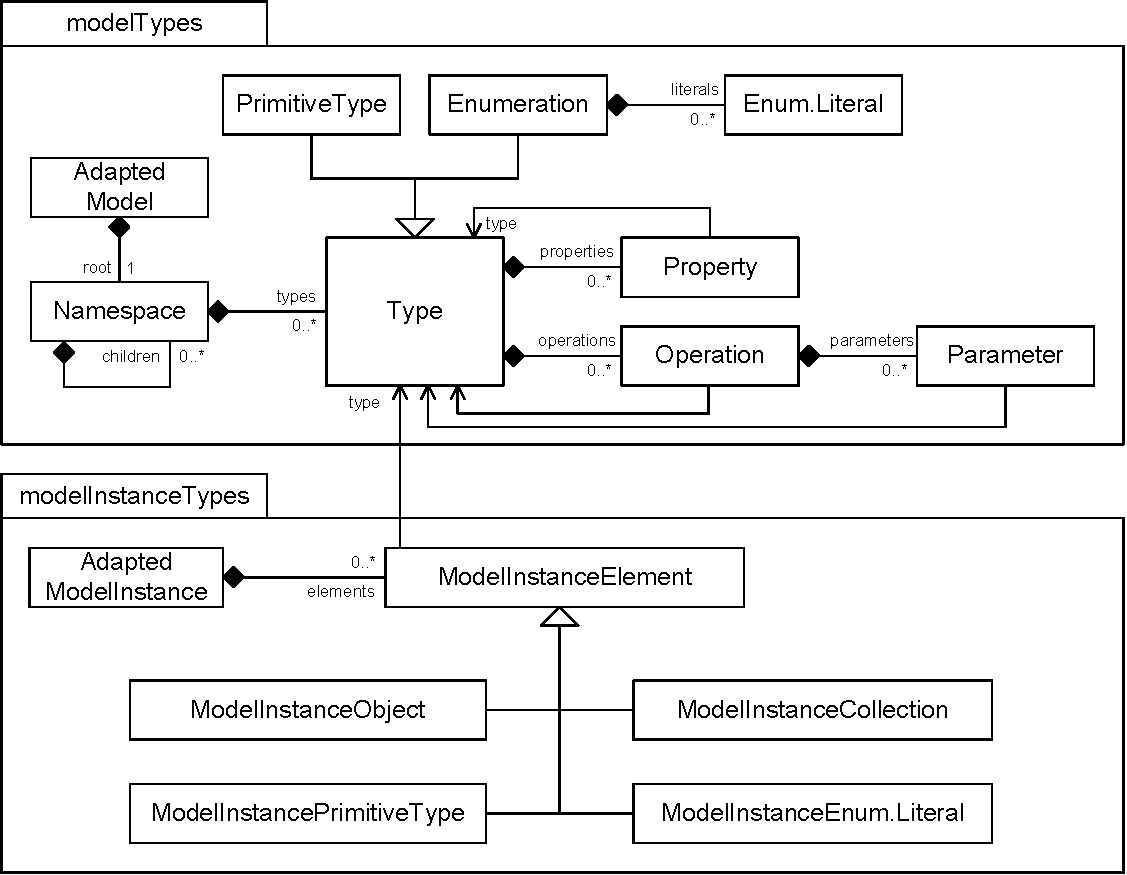
\includegraphics[width=0.80\textwidth]{figures/coreconcepts.pdf}
			\caption{The core concepts of the \emph{Model Types} and \emph{Model Instance Types}:
			Each \emph{Model} has a root \emph{Namespace} that contains a set of nested Namespaces and 
			a set of \emph{Types}. Each Type has a set of \emph{Operations} 
			and \emph{Properties}. 
			Each \emph{Model Instance} has a set of \emph{Model Instance Elements}. Each Model Instance
			Element has exactly one Type and provides 
			operations to reflect on this Type. \emph{Model Instance Objects} provide further reflective 
			operations to get properties and to invoke operations.}
			\label{fig:coreconcepts}
		\end{figure}

\subsection{Model Adaptation}

	\begin{figure}[!t]
			\centering
				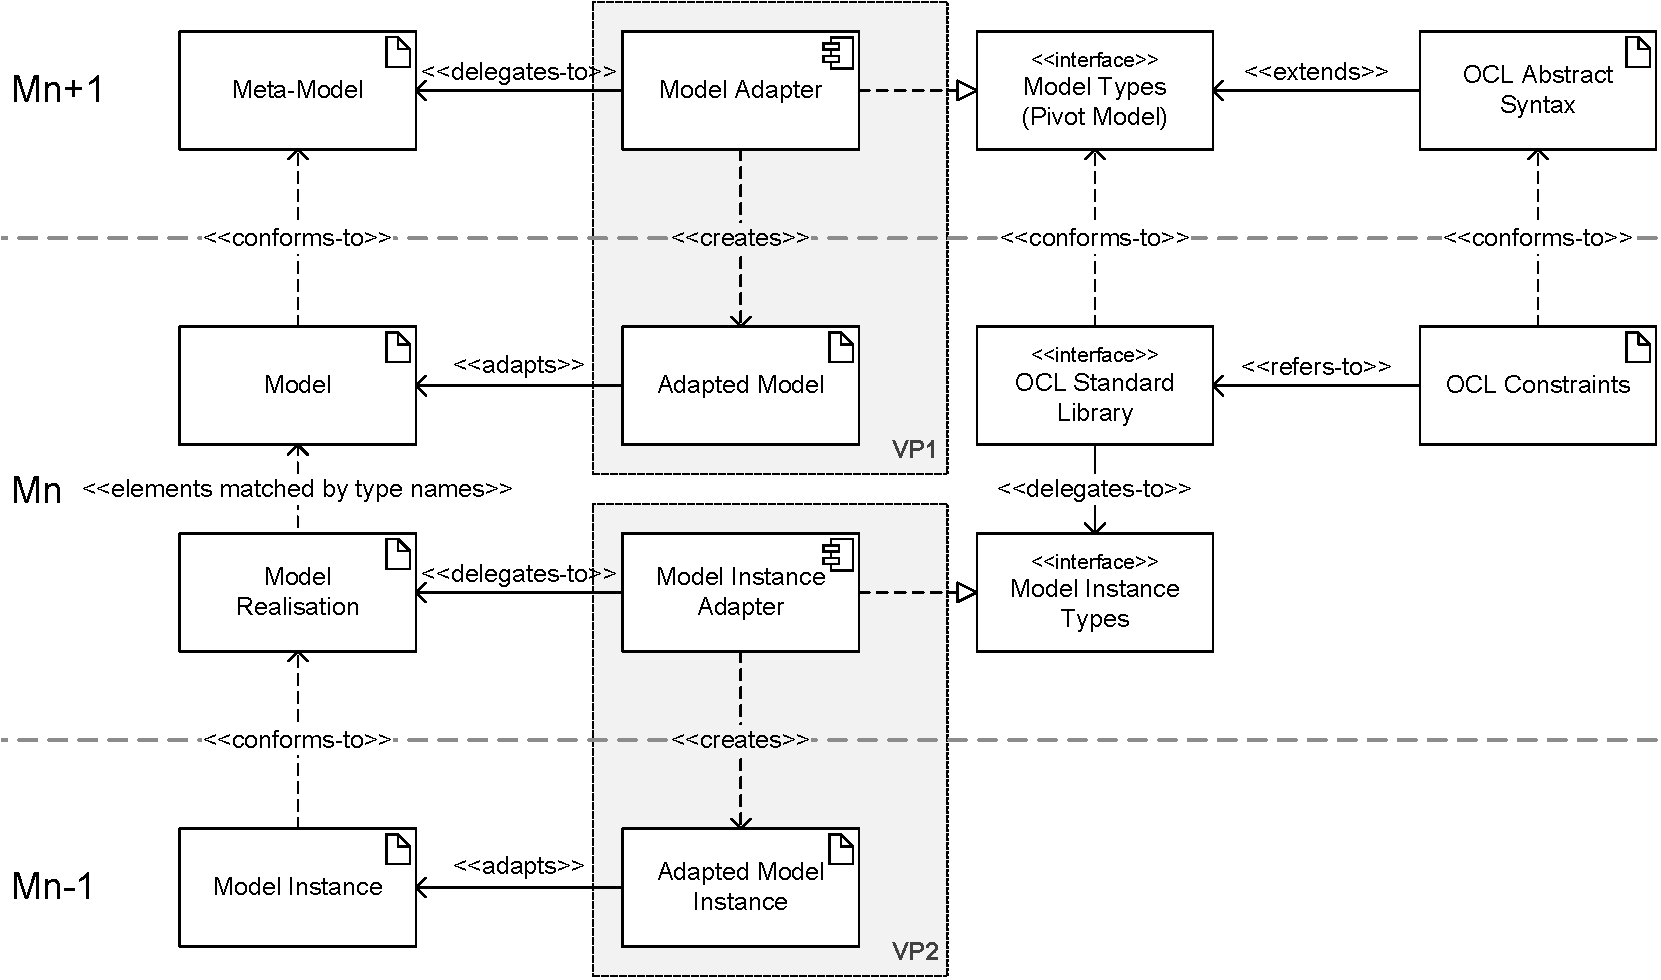
\includegraphics[width=1.00\textwidth]{figures/modeladaptation.pdf}
			\caption{The \emph{Generic Adaptation Architecture} of DresdenOCL: At the Mn+1 layer, meta-models are adapted
			to the model types (VP1). The model adapter component contains these adapters and is responsible 
			to instantiate them to adapt models of the meta-model. 
			At the Mn layer, model implementation types are adapted (VP2). The model instance adapter component
			contains these adapters and is responsible to instantiate them to adapt model instance objects. 
			The OCL standard library implements the logic to evaluate operations defined on OCL types. Other 
			requests such as operation invocations or property requests on adapted objects are delegated 
			via the interfaces of the model implementation type model.}
			\label{fig:modeladaptation}
		\end{figure}

	To enable the definition of OCL constraints for various modelling languages,
	DresdenOCL provides a set of common interfaces abstracting structures
	that are required to navigate and query object structures.
	These interfaces--called \emph{Model Types} (or \emph{Pivot Model}) \cite{braeuerOCL07}--standardize
	the basic	concepts such as types, properties, operations and parameters
	that bind OCL constraints to a concrete modelling language (cf. Fig. \ref{fig:coreconcepts}).
	DresdenOCL only	uses these concepts to parse and statically analyse OCL constraints, 
	e.g., the OCL2 parser	invokes the operation \texttt{getType()} to access the \texttt{Type} of 
	an \texttt{Operation} or \texttt{Property}.
	
	For every meta-model that shall be connected with DresdenOCL, 
	a \emph{Model Adapter} component has to be implemented (cf. Fig. \ref{fig:modeladaptation}, Mn+1 layer). 
	It contains individual adapters that map concepts of the modelling
	language to corresponding artefacts of the model types. E.g., the UML
	meta-model concept \texttt{UMLClass} is adapted to the model type concept
	\texttt{Type} \note{Christian: Again, figure needed. Claas: Fig 2 sufficient?}. 
	Furthermore, the model adapter component has to provide a factory to create 
	adapters on demand resulting in an \textit{Adapted Model} (cf. Fig.
	\ref{fig:modeladaptation}, Mn+1 and Mn layer).
	The adapters are only created for model elements that are required and
	existing adapters are cached. Thus, we avoid unnecessary and expensive adaptation, 
	especially when working on large models of which only parts are constrained using OCL.
	The presented architecture provides a generic and easy variation of multiple meta-models
	and corresponding models in an OCL infrastructure (VP1).


\subsection{Model Instance Adaptation}
	
	The presented abstraction of model types to support various models
	and meta-models can now be shifted and extended to
	solve similar problems when working with multiple model instantiations. Now we
	present the solution addressing the second variation point (VP2) for a generic adaptation
	architecture of an OCL infrastructure.
	
	Similar to the adaptation of different meta-models and models, it is
	useful to hide different model implementations
	behind standardised interfaces. This enables the
	reuse of the same OCL2 interpreter for the dynamic
	evaluation of OCL constraints on model instance elements in various model
	instantiations. To provide means for model
	instance adaptation, we introduced the \emph{Model Instance
	Types}. The model instance types are different
	interfaces for instances of standard types in OCL such as primitive types, 
	collections and objects (cf. Fig. \ref{fig:coreconcepts}). 
	All these	interfaces inherit a common interface \texttt{ModelInstanceElement}. The most 
	important difference between the model types and the model instance types
	is that \texttt{ModelInstanceElements} provide a reflection mechanism whereas 
	model type elements only allow to reason on relationship between concepts of
	the same meta-level. During interpretation, the OCL2 interpreter uses these reflection mechanisms to
	retrieve the \texttt{Type} of a \texttt{ModelInstanceElement}, access \texttt{Property}
	values, or to invoke \texttt{Operations}.
	
	Each kind of model instance that shall be connected with DresdenOCL is
	adapted via a \emph{Model Instance Adapter} component (cf. Fig.
	\ref{fig:modeladaptation}, Mn layer). Similar to the model adapter, 
	the model instance adapter component contains adapters that map elements of a
	concrete model instance to model instance types and has to
	provide a factory that creates \emph{Model Object Adapters} for the runtime 
	objects of the adapted model instance (cf. Fig. \ref{fig:modeladaptation}, Mn-1 layer). 
	Like the model adapter, the model instance adapter also 
	creates adapters for objects on demand. Adapted objects are cached to
	improve the performance and to avoid phenomena like \emph{Object
	Schizophrenia} \note{reference}. Due the introduction of a common set of model
	instance types it is possible to easily reuse the same OCL interpreter
	for various kinds of model instances. Thus, VP2 can be completely addressed
	by the presented generic adapter architecture.


